\subsection{UML-Diagramm}
\label{subsec:uml}

\begin{landsacpe}
\begin{figure}[h]
\centering
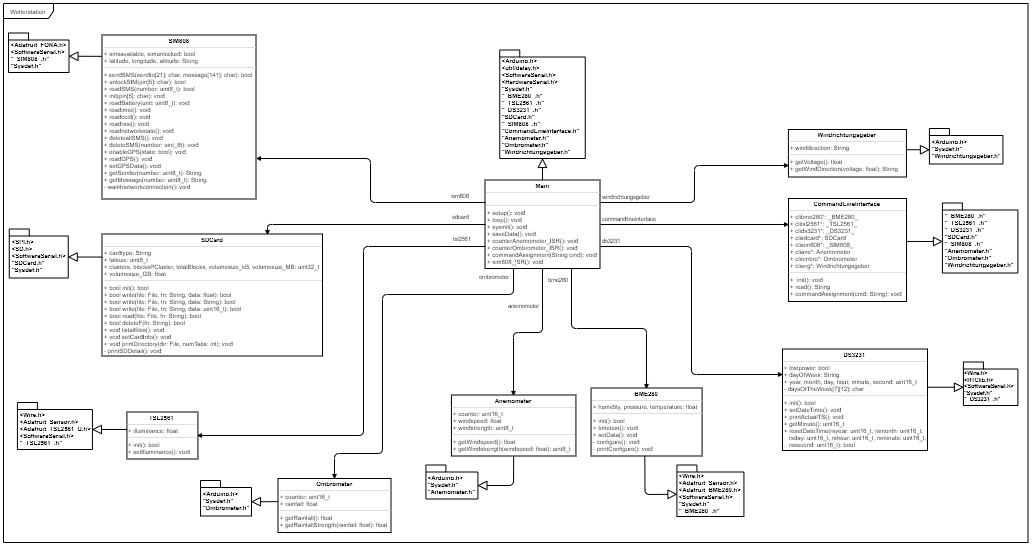
\includegraphics[width=0.9\textwidth]{../../graphics/UML/uml_diagramm_p6.PNG} 
\caption{UML-Diagramm}
\label{fig:uml_diagramm}
\end{figure}
\end{landscape}

Das in der Abbildung \ref{fig:uml_diagramm} dargestellte UML-Diagramm soll den Aufbau und die logischen Zusammenhänge der Firmware visualisieren. Darin wird gezeigt, welche Headerfiles bei den Klassen benötigt werden. Zudem sind die Attribute, wie auch die Funktionen mit ihren Access Specifier, Argumenten und Rückgabewerten aufgelistet. Der Inhalt ist wegen der Skalierung etwas schwierig zu lesen. Deshalb könnte das UML-Diagramm aus dem beigelegten Berichtsordner im \textit{Fachbericht_P6/graphics/UML} auf der Internetseite \url{https://www.draw.io/} per \textit{Open Existing Diagram} geöffnet und genauer angeschaut werden.\\

Durch diese Struktur ist es möglich, adaptiv mehrere Komponenten hinzuzufügen und anzupassen. Zudem könnten somit auch mehrere Sensoren vom gleichen Typ ohne grossen weiteren Aufwand implementiert werden. Daher auch ein Vorteil des verwendeten I$^{2}$C-Interface.\\

Alle Systemrelevanten Definitionen sind im Headerfile Sysdef.h definiert. Damit sind Werte, welche auf das gesamte Projekt übergreifen leicht änderbar.\\

Im Zentrum des Programms steht die \textit{Main}. Sie enthält das Setup, sowie auch den Loop, welcher nach dem Setup kontinuierlich ausgeführt wird. Also äquivalent zu einer while(1){}. Als erstes werden alle Instanzen instanziert, danach im Setup alle an die MCU angeschlossenen Bauteile initialisiert. Der Loop in der Main hat in der aktuellen Implementierung drei Grundaufgaben zu erledigen. Als erstes muss er zeitlich über den DS3231 überprüfen, ob es wieder einen Messzeitpunkt gibt und dann darauffolgend gleich die Messdaten setzt und auf die $\mu$SD-Karte speichert. Zweitens muss er das Commandlineinterface betreiben, rsp. abragen, ob etwas per USB gesendet wurde. Anschließend je nach gültigem Command dann diesen verarbeiten und an die dementsprechende Klasse weiterleiten. Zum Schluss kommt noch die Abrage über eine empfangene SMS. Dafür wurde eine ISR (Interrupt Service Routine) implementiert, welche einen bool smsavailable auf true setzt. Falls dies geschieht, wird aus der SMS der Sender und die Nachricht/Command ausgelesen. Dann werden die zuletzt gespeicherten Daten zurückgesendet und das empfangene SMS wieder gelöscht um wieder Platz zu generieren.\\

\subsubsection{Lizenzen}
\label{subsubsec:lizenzen}

Die verwendeten Librarys sind grundsätzlich aus der Arduino IDE von Arduino. Arduino selbst ist eine aus Soft- und Hardware bestehende Physical-Computing-Plattform, bei welcher beide Komponenten auf Open-Source-Basis quelloffen sind \cite{arduinoWiki}. Nach Aussage von Arduino selbst, stehen alle C/C++ Mikrocontroller Librarys unter der \textbf{LGPL} \cite{ArduinoLicense2019}. Einige Lizenz-Texte stehen im Anhang \ref{sec:lizenztexte}. \\

%Die RTClib steht unter der \textbf{MIT}-Lizenz, zusätzlich befindet sich noch der Lizenz-Text im Anhang \ref{subsec:rtclib_lizenztext}. Auch der Lizenz-Text der Adafruit_BME280 ist im Anhang \ref{subsec:adafruit_bme280_lizenztext}.\\

\begin{table}[h]
\centering
\caption{Lizenzen}
\label{tab:lizenzen}
\begin{tabular}{|l|l|l|}
\hline 
\textbf{Library} & \textbf{Author} & \textbf{Lizenz} \\ 
\hline 
Arduino & Arduino Team & LGPL V2.1 \\ 
\hline 
SPI & Cristian Maglie, Paul Stoffregen, Matthijs Kooijman, Andrew J. Kroll & LGPL V2.1 \\ 
\hline 
Wire & Nicholas Zambetti, Todd Krein, Chuck Todd & LGPL V2.1 \\ 
\hline 
SoftwareSerial & Limor Fried, Mikal Hart, Paul Stoffregen, Garrett Mace, Brett Hagman & LGPL V2.1 \\ 
\hline 
SD & SparkFun Electronics & GPL V3 \\ 
\hline 
RTClib & JeeLabs & - \\ 
\hline 
Adafruit\_Sensor & Kevin Townsend & Apache V2.0 \\ 
\hline 
Adafruit\_BME280 & Kevin Townsend & BSD \\ 
\hline 
Adafruit\_FONA & Limor Fried & BSD \\ 
\hline 
Adafruit\_TSL2561\_U & Kevin Townsend & BSD \\ 
\hline 
\end{tabular} 
\end{table}
\todo[inline]{Schreiben: SD GPL wegen sdfatlib. Es hat da zwei drin, File.cpp und SD.cpp. JeeLabs angeben mit link http://news.jeelabs.org/code/. Die The Android Open Source Project hat bei Adafruit Sensor das Copyright. Vielleicht hinzuschreiben. Und zum schluss noch den Text überarbeiten.}